\documentclass[../../tc_tp3_main.tex]{subfiles}

\begin{document}
\chapter{Introducci\'on a dise\~no de filtros}


Criterios considerados en todos los pasos de la realizaci\'on de filtros:

\begin{itemize}
	\item Cumplir la plantilla con tolerancia del 0\%.
	\item Minimizar la cantidad de componentes. 
	\item Minimizar la cantidad de valores distintos de componentes.
	\item Utilizar un solo valor de inductancia para usar un solo dise\~no de gyrator.
\end{itemize}




\begin{table}[htbp]
\centering
\begin{tabular}{|c|c|c|c|}
\hline 
Tipo de filtro & $f_p[kHz]$ & $f_a[kHz]$ & $f_c[kHz]$ \\ 
\hline 
LP & 4   & 14  & --- \\ 
\hline 
HP & 14  & 4   & --- \\ 
\hline 
BP & --- & --- & 8   \\ 
\hline 
BR & --- & --- & 4   \\ 
\hline 
\end{tabular}
\label{tab:ej2_plantilla} 
\caption{Plantilla}
\end{table}







\section{Dise\~no de funciones transferencias}\begin{tabular}{|c|c|c|c|}
\hline 
Tipo de filtro & $f_p[kHz]$ & $f_a[kHz]$ & $f_c[kHz]$ \\ 
\hline 
LP & 4   & 14  & --- \\ 
\hline 
HP & 14  & 4   & --- \\ 
\hline 
BP & --- & --- & 8   \\ 
\hline 
BR & --- & --- & 4   \\ 
\hline 
\end{tabular} 



\subsection{High-Pass}

R = 1.5k	\\
C = 0.022uF	\\
L = 0.016H	\\
Cut-off frequency	\\
fc = 8482.9869696821[Hz]	\\
Quality factor	\\
Q = 0.56853524361496	\\
Damping ratio	\\
xi = 0.87945295496689	\\

\subsection{Low-Pass}

R = 1.5k \\
C = 0.022uF \\
L = 0.016H \\
Cut-off frequency \\
fc = 8482.9869696821[Hz] \\
Quality factor \\
Q = 0.56853524361496 \\
Damping ratio \\
xi = 0.87945295496689 \\

\subsection{Band-Pass}

\subsection{Band-Reject}

\section{EL POR QUE DE LA CANTIDAD DE INTEGRADOS Y SMD}

ELEGI DOS INTEGRADOS DE 4 AUNQUE PODRIA HABER USADO UNO DE 4 Y UNO DE 2 PARA SEPARAR LOS GYRATORS DE LOS DEL RESTADOR. SI POSTA QUERES USAR UN SOLO INTEGRADO, O TE BANCAS LA SALIDA DIFERENCIAL Y ELIMINAL EL INTEGRADO DEL RESTADOR, O TE COMPRAS UNO DE 6 OPAMPS QUE EXISTEN Y TIENEN BANDA ANCHA (10MHZ).

ELEGI SMD PORQUE SI NO NO ME DABA EL MONTECARLO PARA HACER EL LP Y EL HP JUNTOS.

\section{SALIDA DIFERENCIAL DEL LP}


Como se ve en las figuras \ref{fig:ej2_LP_gyr_res_vs_dif} y \ref{fig:ej2_LP_rlc_res_vs_dif}, hay bocha de diferencia si uso el restador o si no lo uso, pero me empieza a joder arriba de la frecuencia maxima a la cual el gyrator anda piola (aprox 20k).

\begin{figure*}[htbp]
\centering
	\includegraphics[width=0.7\textwidth]{imagenes/{"LP_gyr no res vs LP_gyr"}}
	\label{fig:ej2_LP_gyr_res_vs_dif}
	\caption{Simulaci\'on del fitro low-pass con bobina real tomando salida diferencial y usando el restador }
\end{figure*}

\begin{figure*}[htbp]
\centering
	\includegraphics[width=0.7\textwidth]{imagenes/{"LP_rlc no res vs LP_rlc"}}
	\label{fig:ej2_LP_rlc_res_vs_dif}
	\caption{Simulaci\'on del fitro low-pass con bobina real tomando salida diferencial y usando el restador }
\end{figure*}

\section{Gyrator}

\subsection{Uso como simulador de un inductor. Limitaciones en frecuencia.}

\begin{figure*}[htbp]
	\centering
	\begin{circuitikz}[scale=1]
%\draw[help lines]   			grid(6,6);	
\draw								(0,3)
		to [R=$R_L$,i>^=$i_{in}$]	(3,3)
		to [L=$L{=}R_LRC$]			(3,0) node[ground]{};
\end{circuitikz}

	\begin{circuitikz}[scale=1]
\draw[help lines]   			grid(6,6);	

\draw									(0,3)
		to [short, o-*, i>^=$i_{in}$]	(1,3)
		to [short, i>_=$i_A$]			(1,4)
		to [R=$R_L$]				(3,4)
		to [short] 					(3,5)
		to [short]					(5.5,5)
		to [short]					(5.5,3.5)

									(3,2)
		to [short]					(3,3)
									(1,3)
		to [short, i>^=$i_B$]		(1,2)
		to [C=$C_1$]				(3,2)
		to [R=$R_1$]				(3,0) node[ground]{}
		
									(4.25,3.5)
		node[op amp](opamp){};
\end{circuitikz}

	\caption{Uso de gyrator como inductor}
	\label{fig:ej2_gyrator_simulacion_inductor}
\end{figure*}


\subsubsection{Obtenci\'on impedancia de entrada $Z_{in}$}

Para el siguiente c\'alculo se desprecian las corrientes de bias y la tensi\'on de offset.\\

Relaci\'on entre $V^-$ y $V^+$:
\begin{align}
V^- &= A_{vol}\left( V^+ - V^-  \right)	\\
V^- \left( 1 + A_{vol}\right) &= A_{vol}\, V^+ \\
V^- &= V^+\frac{A_{vol}}{1+A_{vol}}\\
V^- &= V^+K \label{eq:ej2_relacion_entradas_opamp_gyrator}
\end{align}

Con $K=\frac{A_{vol}}{1+A_{vol}}$.
Usando el modelo de $A_{vol}$ del polo dominante se obtiene la expresion de K:

%relaicion entre V- y V+
\begin{align}
K&= \frac{\frac{A_o}{\frac{s}{\omega_p}+1}}{\frac{A_o}{\frac{s}{\omega_p}+1}+1} \\
 &= \frac{A_o}{(A_o + 1) + \frac{s}{\omega_p}}\\
 &= \frac{A_o}{A_o+1} \cdot \frac{1}{1+\frac{s}{(A_o+1)\omega_p}}\\
 \intertext{Considerando que $A_o+1\approx A_o$:}
  &=\frac{1}{1+\frac{s}{BWP}}
 \intertext{Siendo $BWP=A_o\cdot \omega_p$}
\end{align}
\todo{BWP es con 2pi o sin?}

Se buscan las tensiones en las entradas del \textit{op-amp} para luego hallar las corrientes $i_A$ y $i_B$.


%relacion de V- y V+ con Vin
\begin{align}
	\intertext{Por divisor resistivo:}
	V^+&=V_{in}\frac{R_1}{R_1+\frac{1}{sC}} \\
	\intertext{De la ecuaci\'on \ref{eq:ej2_relacion_entradas_opamp_gyrator}:}
	V^-&=V_{in}\cdot K \frac{R_1}{R_1+\frac{1}{sC}}
\end{align} 

%i_A
\begin{align}
i_A &= \frac{1}{R_L}\left(V_{in} - V^-\right)\\
 &= V_{in} \frac{1}{R_L}\left( 1-K\frac{R_1}{R_1+\frac{1}{sC}} \right)\\
 &= V_{in} \frac{sCR_1+1-KsCR_1}{R_L\left( sCR_1+1 \right)} \\
 &= V_{in} \frac{(1-K)sCR_1+1}{R_L\left( sCR_1+1 \right)}
\end{align}


%i_B
\begin{align}
i_B &= V_{in} \frac{1}{\frac{1}{sC} + R_1}\\
	&= V_{in} \frac{sC}{1+sCR_1}
\end{align}

%i_{in}
\begin{align}
i_{in} &= i_A + i_B \\
 &= V_{in} \left( \frac{(1-K)sCR_1+1}{R_L\left( sCR_1+1 \right)} +   \frac{sC}{1+sCR_1}   \right) \\ 
 &= V_{in}  \frac{(1-K)sCR_1+1 + sCR_L}{R_L\left( sCR_1+1 \right)} \\
 &= V_{in}  \frac{sC(R_1(1-K)+R_L) + 1}{R_L(sCR_1+1)} 
\end{align}

De este resultado se obtiene la impedancia de entrada:

\begin{equation}
Z_{in}= \frac{ sCR_1R_L+R_L}{sC(R_1(1-K)+R_L) + 1}
\end{equation}


%condiciones para la aproximacion
\begin{description}
	\item [\textbf{$K \approx 1$}] Elijo criterio: K tiene la forma de una transferencia de un filtro pasabajos de primer orden. Siendo $f_0$ la frecuencia de corte, se considera que $K\approx 1$ si $f<\frac{f_0}{10}$, es decir, una d\'ecada antes de la frecuencia de corte. En este caso, $f_0=BWP$ y la aproximaci\'on es v\'alida para $f<\frac{BWP}{10}$
	
	\item [\textbf{$sCR_L +1 \approx 1$}] Elijo criterio: $2\pi fCR_L <0.05 \iff f< \frac{0.05}{2\pi CR_L}$
\end{description}

La restricci\'on de BWP es independiente de la eleccion de componentes, osea que es fija. busco con la eleccion de componentes que la otra restriccion sea mas laxa que la primera para que funcione durante mas frecuencia.

Usando TL082 con $BWP=8MHz$:
\begin{align*}
\frac{BWP}{10} \leqslant \frac{0.05}{2\pi C R_L} \\
\Rightarrow CR_L\leqslant \frac{1}{4\pi BWP} \approx 20ns
\end{align*}




Si la frecuencia cumple con las dos condiciones anteriores, la impedancia de entrada se puede aproximar a la del modelo de un inductor con resistencia serie con valores $L=CR_LR_1$ y $R_{coil}=R_L$

\begin{align}
	Z_{in} &= sCR_LR+R_L \\
 	\abs{Z_{in}} &= R_L \, \sqrt{4\pi^2f^2C^2R^2+1} \\
 	\phase{Z_{in}} &= arctg(2\pi fCR)
	\label{eq:ej2_zin_gyrator_con_aprox}
\end{align}

Observar que $R_1$ no tiene restricciones sobre qu\'e valores puede tomar para que el gyrator se comporte como un inductor, no afecta a la resistencia serie final, y si afecta a la L, osea que es el valor clave para modificar 

 

\subsection{Criterios de dise\~no}

\begin{enumerate}
	\item Elijo $CR_L < \frac{1}{4\pi BWP}$
	\item Elijo $R_L < \frac{Rcircuito}{20}$. De ahi obtengo $C$
	\item Elijo $Rgyrator = \frac{L}{CR_L}$
\end{enumerate}






\subsection{Otras limitaciones}

\begin{description}
	\item[Funcionamiento a altas y bajas frecuencias]
	\todo[inline]
	
	\item[Alamcenamiento energ\'etico] no puede almacenar energ\'ia de la misma manera que un inductor. La magnitud de la fem producida ante cambios de corriente $\left( V = \frac{di}{dt} \right) $ tiene limitaciones propias de las caracter\'isticas el\'ectricas del circuito (ej.: op-amp no puede largar 100.000kV a pesar de lo que diga spice) 
	\item[Terminal a tierra] una de las terminales del inductor simulado siempre debe estar a tierra \todo{no entiendo cmo se relaciona esto con el modelo de gyrator como cuadripolo que dio dani}
	
	\item[Propiedades magn\'eticas] No crean campos magn\'eticos de la misma forma que los inductores, por lo que no se puede conseguir un efecto de mutua inducci\'on. \footnote{por eso no se puede hacer un transformador con desacople el\'ectrico como si se puede hacer con bobinas posta. Si se puede hacer un transformador poniendo dos en cascada pero es no tiene nada que ver y no hay desacople el\'ectrico. Desacople el\'ectrico es un t\'ermino que existe o o invente?}
	
	\item[ddddd] un transformador implementado con gyrators no tiene aislaci\'on el\'ectrica como si tiene un transformador real. Por ejemplo, no se podr\'ia implementar un transformador de aislaci\'on \todo{traduccion de isolation transformer esta bien?}

\end{description}




\section{An\'alisis de resultados}

\subsection{High-pass}

Se muestra la respuesta calculada, simulada y medida en la figura \ref{fig:ej2_HP_bode}. La respuesta calculada se separa de la simulada y la medida en los mismos rangos en que la imepdancia de entrada del gyrator calculada se separa de la simulada.

\begin{figure*}
	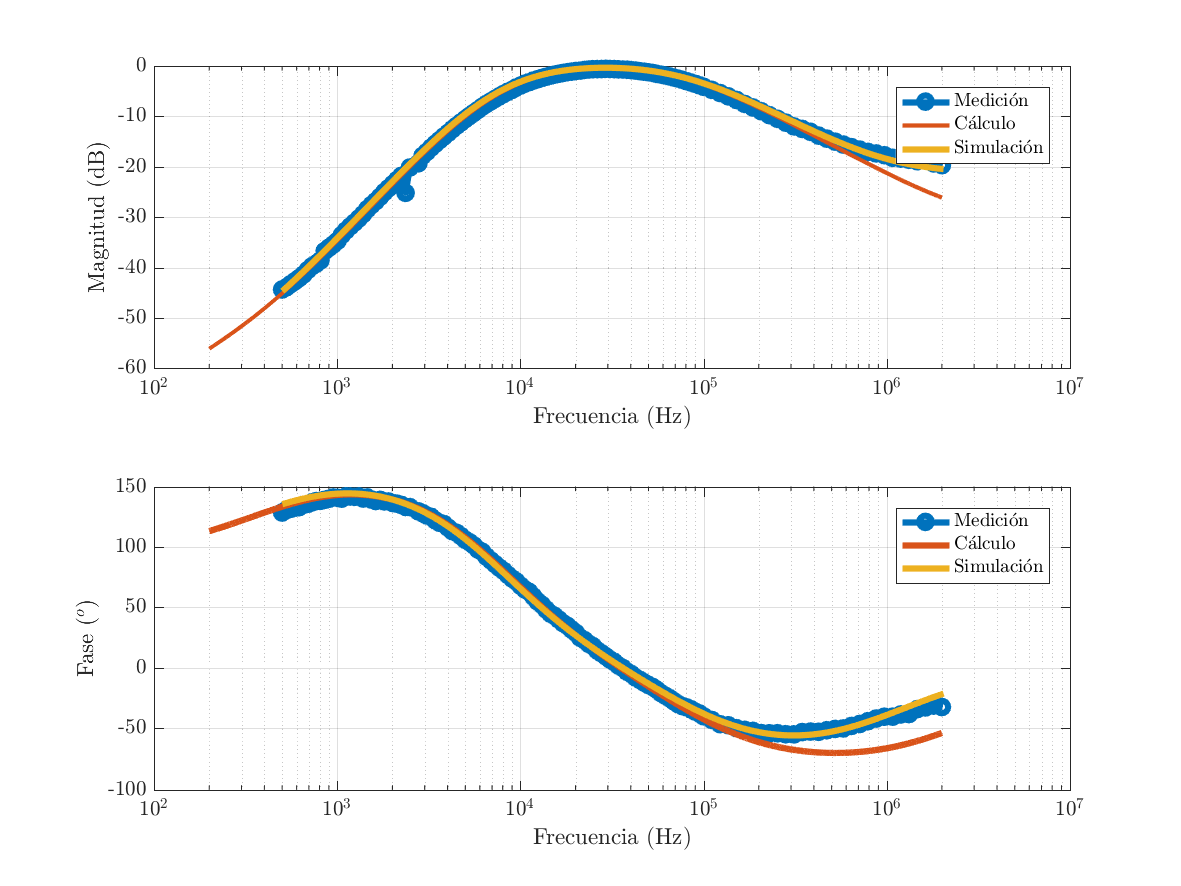
\includegraphics[width=0.7\textwidth]{imagenes/HP_bode}
	\caption{Respuesta en frecuencia del filtro high-pass calculada, simulada, y medida}
		\label{fig:ej2_HP_bode}
\end{figure*}

%\subsection{Low-pass}
%\ref{fig:ej2_LP_bode}
%\begin{figure*}
%	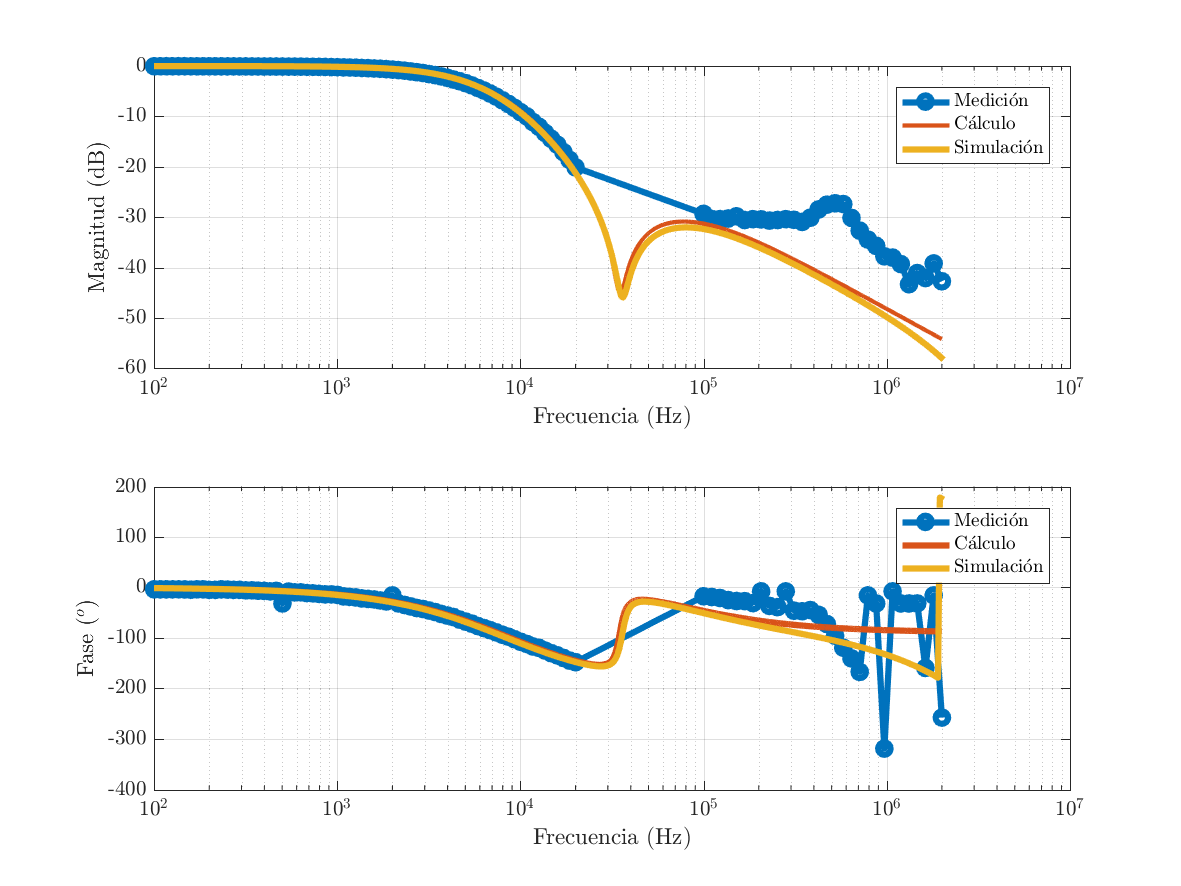
\includegraphics[width=\textwidth]{imagenes/LP_bode}
%	\caption{Respuesta en frecuencia del filtro low-pass calculada, simulada, y medida. El caculo fue hecho para salida diferencial, y la simulacion y la medicion para la salida del restador}
%		\label{fig:ej2_LP_bode}
%\end{figure*}


\subsection{Band-pass}

Se muestra la respuesta calculada, simulada y medida en la figura \ref{fig:ej2_BP_bode}. La respuesta calculada no se separa de la simulaci\'on como si lo hacia la del high-pass, ya que en ese rango de frecuencias el valor del paralelo de capacitor y el inductor esta dominado por el capacitor.

\ref{fig:ej2_BP_bode}
\begin{figure*}
	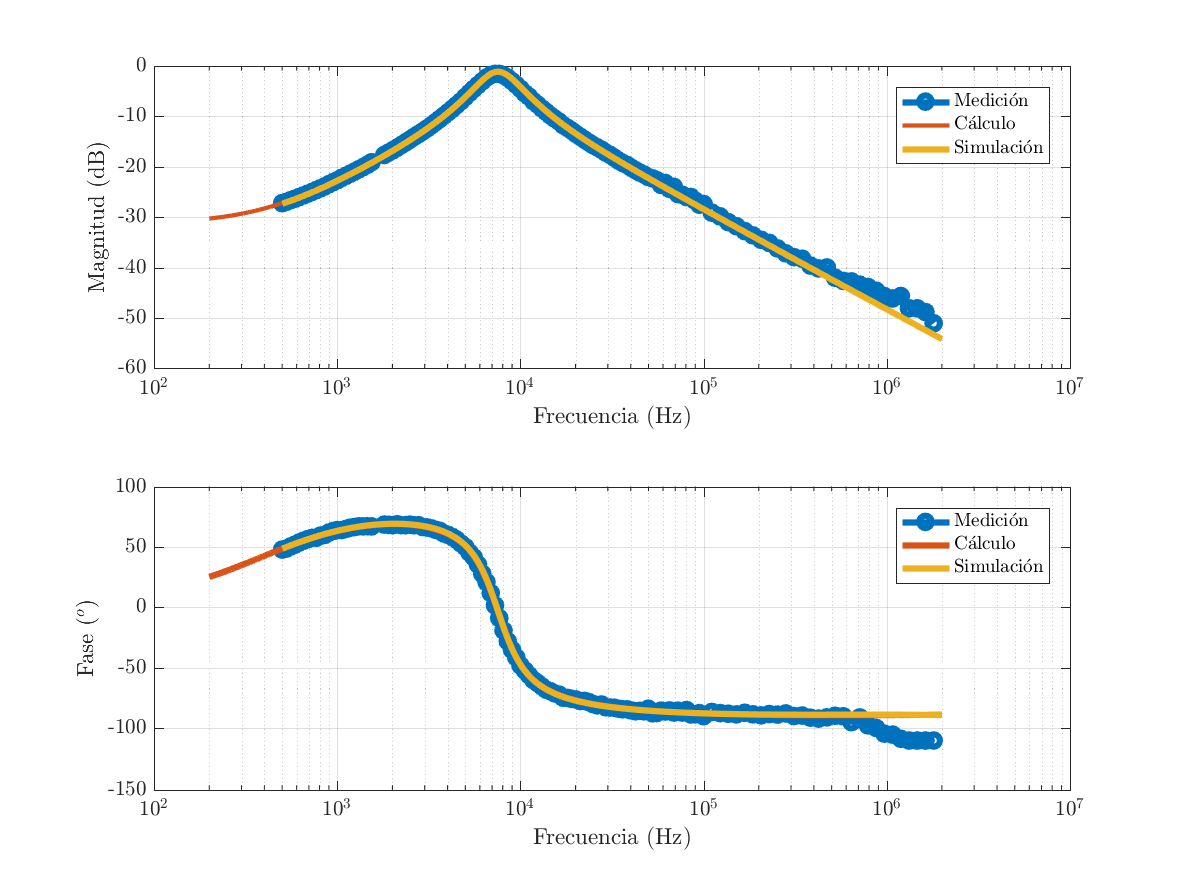
\includegraphics[width=0.7\textwidth]{imagenes/BP_bode}
	\caption{Respuesta en frecuencia del filtro band-pass calculada, simulada, y medida}
		\label{fig:ej2_BP_bode}

\end{figure*}


\subsection{Band-reject}

Se muestra la respuesta calculada, simulada y medida en la figura\ref{fig:ej2_BR_bode}. Se repite la diferencia de comportamiento entre la respuesta calculada, y la simulada y medida del filtro high-pass. 
\begin{figure*}
	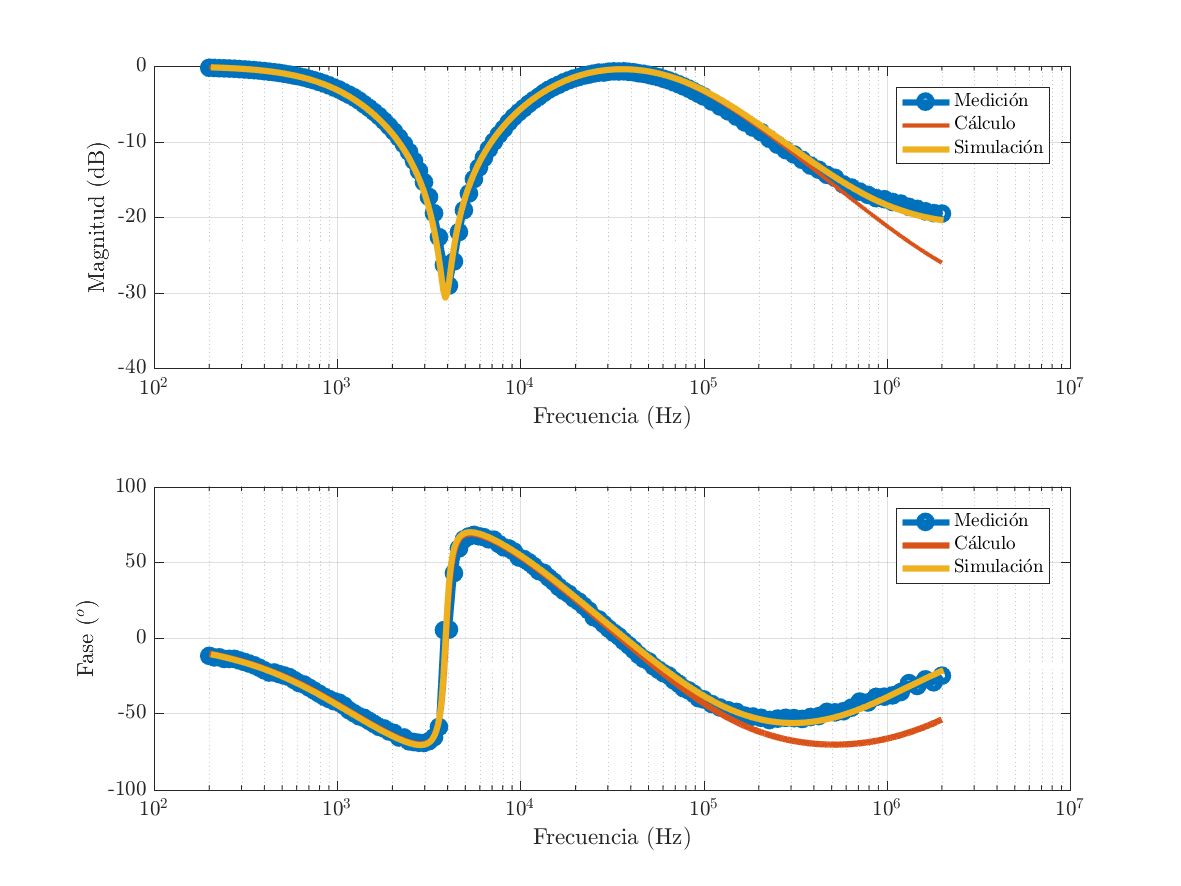
\includegraphics[width=0.7\textwidth]{imagenes/BR_bode}
	\caption{Respuesta en frecuencia del filtro band-reject calculada, simulada, y medida}
		\label{fig:ej2_BR_bode}

\end{figure*}



\section{Anexo}

\subsection{Obtenci\'on funciones transferencia RLC ideal}
\label{ssec:ej2_H_rlc_ideal}

Para todos los filtros se considera 
\begin{align*}
\omega_0 &= \frac{1}{\sqrt{LC}}\\
\alpha &=\frac{R}{2L}\\
\xi &= \frac{\alpha}{\omega_0} \\ &= \frac{R}{2}\sqrt{\frac{C}{L}} \\
Q&=\frac{1}{2\xi} \\ &= \frac{1}{R}\sqrt{\frac{C}{L}}
\end{align*}

\subsubsection{Filtro high-pass}

RLC serie tomando la salida en el capacitor:

\begin{align}
H(s)&=\frac{\frac{1}{sC}}{\frac{1}{sC}+R+sL}	\\
&= \frac{1}{s^2 \, LC + s\, RC + 1}	\\
&= \frac{1}{\left(\frac{s}{\omega_0}\right)^2 + \frac{s}{\omega_0}\, 2\xi + 1}
\end{align}


\subsubsection{Filtro low-pass}

$RLC$ serie tomando la salida en el inductor:

\begin{align}
H(s)&=\frac{sL}{\frac{1}{sC}+R+sL}	\\
&= \frac{s^2LC}{s^2 \, LC + s\, RC + 1}	\\
&= \frac{\left(\frac{s}{\omega_0}\right)^2}{\left(\frac{s}{\omega_0}\right)^2 + \frac{s}{\omega_0}\, 2\xi + 1}
\end{align}

\subsubsection{Filtro band-reject}

$RLC$ serie tomando la salida en el inductor y el capacitor:

\begin{align}
H(s)&=\frac{sL + \frac{1}{sC}}{\frac{1}{sC}+R+sL}	\\
&= \frac{s^2LC+1}{s^2 \, LC + s\, RC + 1}	\\
&= \frac{\left(\frac{s}{\omega_0}\right)^2+1}{\left(\frac{s}{\omega_0}\right)^2 + \frac{s}{\omega_0}\, 2\xi + 1}
\end{align}

\subsection{Obtenci\'on impedancia de entrada $Z_{in}$} \label{ssec:ej2_obtencion_zin_gyr}

Para el siguiente c\'alculo se desprecian las corrientes de bias y la tensi\'on de offset.\\

Relaci\'on entre $V^-$ y $V^+$:
\begin{align}
V^- &= A_{vol}\left( V^+ - V^-  \right)	\\
V^- \left( 1 + A_{vol}\right) &= A_{vol}\, V^+ \\
V^- &= V^+\frac{A_{vol}}{1+A_{vol}}\\
V^- &= V^+K \label{eq:ej2_relacion_entradas_opamp_gyrator}
\end{align}

Con $K=\frac{A_{vol}}{1+A_{vol}}$.
Usando el modelo de $A_{vol}$ del polo dominante se obtiene la expresion de K:

%relacion entre V- y V+
\begin{align}
K&= \frac{\frac{A_o}{\frac{s}{\omega_p}+1}}{\frac{A_o}{\frac{s}{\omega_p}+1}+1} \\
 &= \frac{A_o}{(A_o + 1) + \frac{s}{\omega_p}}\\
 &= \frac{A_o}{A_o+1} \cdot \frac{1}{1+\frac{s}{(A_o+1)\omega_p}}\\
 \intertext{Considerando que $A_o+1\approx A_o$:}
  K&=\frac{1}{1+\frac{s}{2\pi BWP}}	\label{eq:ej2_K}
 \intertext{Siendo $2\pi BWP=A_o\cdot \omega_p$}
\end{align}


Se buscan las tensiones en las entradas del \textit{op-amp} para luego hallar las corrientes $i_A$ y $i_B$.

%relacion de V- y V+ con Vin
\begin{align}
	\intertext{Por divisor resistivo:}
	V^+&=V_{in}\frac{R_{gyr}}{R_{gyr}+\frac{1}{sC_{gyr}}} \\
	\intertext{De la ecuaci\'on \ref{eq:ej2_relacion_entradas_opamp_gyrator}:}
	V^-&=V_{in}\cdot K \frac{R_{gyr}}{R_{gyr}+\frac{1}{sC_{gyr}}}
\end{align} 

%i_A, i_B, i_A+i_B
\begin{align*}
i_A &= \frac{1}{R_L}\left(V_{in} - V^-\right)\\
 &= V_{in} \frac{1}{R_L}\left( 1-K\frac{R_{gyr}}{R_{gyr}+\frac{1}{sC_{gyr}}} \right)\\
 &= V_{in} \frac{sCR_{gyr}+1-KsC_{gyr}R_{gyr}}{R_L\left( sC_{gyr}R_{gyr}+1 \right)} \\
 &= V_{in} \frac{(1-K)sC_{gyr}R_{gyr}+1}{R_L\left( sC_{gyr}R_{gyr}+1 \right)}\\
 & \\
i_B &= V_{in} \frac{1}{\frac{1}{sC_{gyr}} + R_{gyr}}\\
	&= V_{in} \frac{sC_{gyr}}{1+sC_{gyr}R_{gyr}}\\
 & \\
i_{in} &= i_A + i_B \\
 &= V_{in} \left( \frac{(1-K)sC_{gyr}R_{gyr}+1}{R_L\left( sC_{gyr}R_{gyr}+1 \right)} +   \frac{sC_{gyr}}{1+sC_{gyr}R_{gyr}}   \right) \\ 
 &= V_{in}  \frac{(1-K)sC_{gyr}R_{gyr}+1 + sC_{gyr}R_L}{R_L\left( sC_{gyr}R_{gyr}+1 \right)} \\
 &= V_{in}  \frac{sC_{gyr}(R_{gyr}(1-K)+R_L) + 1}{R_L(sC_{gyr}R_{gyr}+1)}
\end{align*}

De este resultado \ref{eq:ej2_iin_gyr} se obtiene la impedancia de entrada:

\begin{equation}
	Z_{in}= \frac{ sCR_{gyr}R_L+R_L}{sC_{gyr}(R_{gyr}(1-K)+R_L) + 1} \label{eq:ej2_zin_gyr_sin_aprox} \\
\end{equation}
	en donde	$K  \approx\frac{1}{1+\frac{s}{2\pi BWP}}$ (ecuaci\'on \ref{eq:ej2_K}).



\end{document}
